\chapter{Context}
\label{Context}
\thispagestyle{empty}


This thesis work takes place in the scope of autonomous driving applied in virtual environments, i.e. videogames and simulators. In particular, our goal is to design an autonomous driver able to achieve competitive lap-time compared to human drivers. This task is a key problem in real-world car racing as well as in the development of non-player characters for a commercial racing game. The optimal racing line is defined as the line to follow to achieve the best lap-time possible on a given track with a given car.
Autonomous racing in videogames in a common practice since the birth of the first videogames consoles in the '90s. Sony, Namco, Electronic Arts are just some names of the most active and notorious commercial distributors of the most played racing videogames. Along with the evolution of technology, virtual driving styles have seen constant improvement in human-like skills. Over the years, the so called "bots" have improved their driving capabilities reflecting the state-of-the art theoretical and technological innovations that the scientific community contributed to.
The latest promising topic in this field is Machine Learning, and in particular Reinforcement Learning, which is based on an agent learning from its errors to improve its performance. We will discuss these techniques in detail in the next chapters. However, the state-of-the art technologies upon which autonomous driving is based on more traditional AI algorithms, which involves expert's rules encoded into the program, while Machine Learning solutions are still at research and experimentation stage.
To address the challenge of autonomous racing, we chose to adopt a simulator. 
This is due to many reasons: a simulator is much simpler than the real world, and the task we are going to address is much more easy to manage in a controlled environment such as a simulator.
Safety is another aspect to take into consideration: training an autonomous vehicle involves a lot of trial-and-error, and an error could be very dangerous -if not fatal- especially at the speed that racing cars typically go.
Finally, training an autonomous vehicle in the real world is a long and costly operation: it involves a car racing a lot of times, and a computer elaborating data with energy-consuming GPUs.
Using a simulator is a sensitive choice for training, in order to deploy afterwards the final algorithm in a real-world scenario. 
However, transferring the policy obtained by means of a simulator to the real world is a hard task, due to the intrinsic differences between them, which makes the real world far more complex than a simulator. For instance, the computed parameters of the equations ruling the world and the actions to fulfill a task may be different compared to the real ones, thus they may need some fine tuning when embodied into the machine. This is due to the approximations and all the aspects which are not taken into account by the model of the simulator.
Today there exist several racing-oriented driving simulators, along with development environments. Some examples are AWS Deep Racer \cite{deepracer}, TORCS, Racer \cite{carsim}.

\section{TORCS}
TORCS \cite{TORCS}, The Open Racing Car Simulator, is an Open Source car racing simulator. The TORCS project was originally created by Eric Espié and Christophe Guionneau and it is now continued by Bernhard Wymann, Christos Dimitrakakis and other collaborators. This simulator, written in C++, allows the user to drive and to develop automatic drivers, called robots or bots. A bot can control a car using gas and brake pedals, gear shift and steering wheel. TORCS features a detailed physics engine that presents realistic aerodynamics, wheel properties, damage and collision model, etc. The gameplay allows different types of races and a wide range of different tracks and vehicles and it provides a rather sophisticated 3-D graphics for visualization. For this reasons TORCS is not only used as game and has also become quite widespread as research platform in the field of car racing.

TORCS comes as a standalone application in which robots are programmed in C++, so it restricts the choice of the programming language. Very useful for the scientific community proved to be the work of Loiacono et al. \cite{SCRC} for the 2009 Simulated Car Racing Championship. Their software for the competition extends the original TORCS architecture structuring it as a client-server application: the driving algorithm can run separately from TORCS and can communicate with its server through UDP connection. The server job is to send information of the TORCS environment to the client, receive the action and apply it to the environment.
Figure~\ref{fig:torcs-arc} shows the software architecture. Server bots manage the connections with external clients through UDP. This extension enables programmers to use different programming languages, different than C++, more suitable for their needs.

For this thesis, we use TORCS version 1.3.7. For interfacing with the simulator we use SnakeOil: it is a Python library that manages the UDP connection with the server, enabling an agent (or driver) to act as client bot in the client-server architecture. It takes care of receiving the information coming from the server, pre-processing it in order to be ready for our agent and sending back the computed action to control the car.

The competition architecture creates a separation between the simulator and the agent. What the driver perceives of the racing environment and the available actions are defined in the server bot. The server sends to the client, via the UDP, a list of virtual sensor-readings (e.g., the track, the speed) that measure the environment. The agent receives the sensor-reading as input and responds with a computed action to control the car. Then it is the server job to actuate it on the environment. The actions available to control the car are a rather typical set of actuators, i.e., the steering wheel, the gas and break pedals and the gearbox.

\begin{figure}[t]
 \centering
  \captionsetup{width=10cm}
  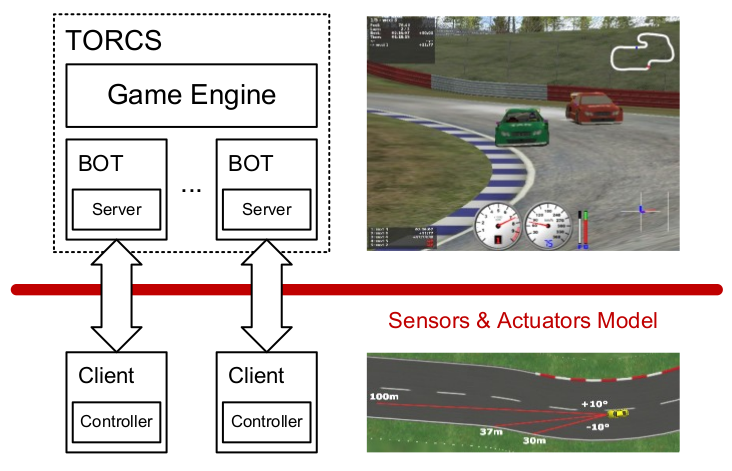
\includegraphics[width=10cm]{./img/torcs_arc}
  \caption{client-server architecture of TORCS}
   \label{fig:torcs-arc}
\end{figure}




